% This syllabus template was created by:
% Brian R. Hall
% Assistant Professor, Champlain College
% www.brianrhall.net

% Document settings
\documentclass[11pt]{article}
\usepackage[margin=1in]{geometry}
\usepackage[pdftex]{graphicx}
\usepackage{multirow}
\usepackage{setspace}
\pagestyle{plain}
\setlength\parindent{4pt}

\begin{document}

% Course information
\begin{tabular}{ l l }
  & \LARGE \textbf{CS 1501} \\\\
  & \LARGE \textbf{Metaprogramming} \\
\end{tabular}
\vspace{10mm}

% Professor information
\begin{center}
\begin{tabular}{ l l }
  \multirow{6}{*}{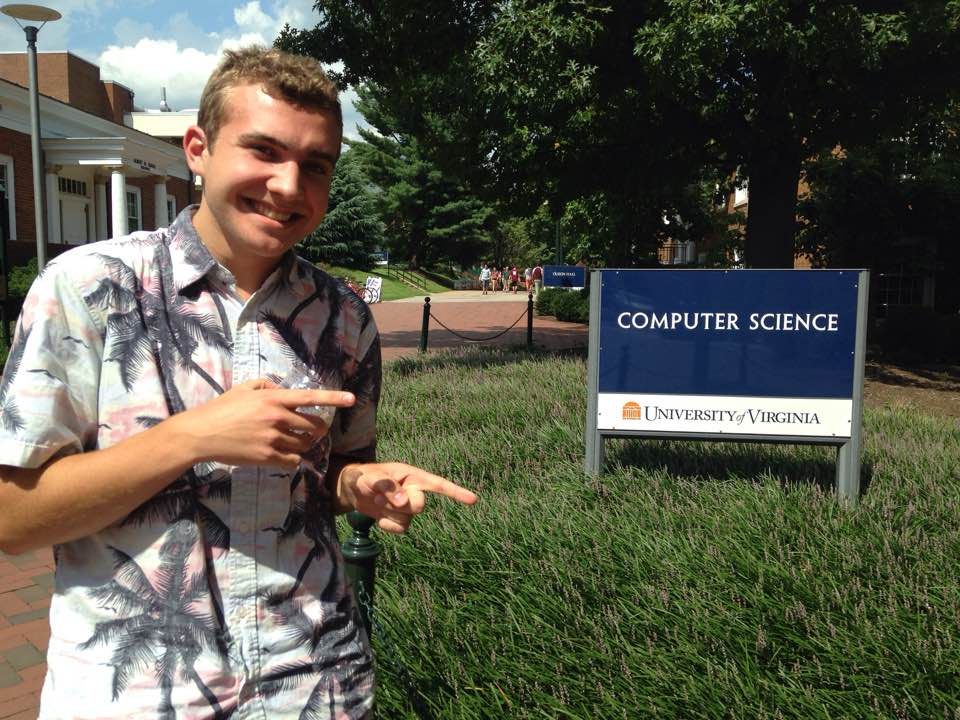
\includegraphics[height=1.85in,width=2.5in]{14040198_10154458676878599_2951113492452685662_n.jpg}} & \\ \\
  & \textbf{\large Maxwell Patek} \\
  & \hspace{2mm} \large mtp4be@virginia.edu \\\\
  & \large \textbf{Office Hours:} \\
  & \hspace{2mm} \large TBD\\
  & \hspace{2mm} \large TBD\\
\end{tabular}
\end{center}

\vspace{10mm}


% Course details
\textbf {\large  Course Description:} Students will learn several implementations and applications of metaprogramming, starting with Python and eventually moving to other languages. Metaprogramming is the writing of programs that take in programs as input and output programs as a result. Metaprograms can sometimes even do this to themselves. Some languages, like Python, have built in features that facilitate this programming style. After this course, students will know these features, what they can accomplish, and the true power of python. More broadly, students will learn how to live DRY (don't repeat yourself). \\

\textbf {Prerequisites:}  
CS 111x and 2110, 
or Familiarity with Object Oriented Programming and Python

\textbf {Credit Hours:} 1 \hspace{5mm} \textbf{Time:} Mondays 1:00 pm \hspace{5mm} \textbf{Room:} Chemical \textit{Engineering} Building 005 \\

\textbf {\large Course Objectives:} \\
At the completion of this course, students will be able to:
\begin{enumerate} \itemsep-0.4em
  \item Write object-oriented Python
  \item Use functions as first-class objects
  \item Use Python Inheritance  
  \item Write closures and decorators
  \item Use and write metaclasses  
  \item Write dynamic classes and functions 
  \item Use reflection in several languages
  \item Understand homoiconicity
  \item Conceptualize intepreters, compilers and specializers as metaprograms
  \item Use compile-time computation
\end{enumerate}

\textbf {\large Grade Distribution:} \\
\hspace*{40mm}
\begin{tabular}{ r l }
Assignments & 50\% \\
Final Exam  & 10\% \\
Attendance  & 40\%
\end{tabular} \\\\

\newpage

\textbf {\large Course Policies:}
\begin{itemize}
	\item \textbf {Lecture}
		\begin{itemize}
			\item Lectures will be integrated lecture-lab. ie mix of instruction and workshop style coding. 
			\item When coding, students should have their computers out; however, I do ask that students keep computers away otherwise. 
			\item There will be minimal need for taking notes, as I will make all lecture materials available on Collab.
		\end{itemize}
		\item \textbf {Assignments}
		\begin{itemize}
			\item There will be an assignment for most weeks. 
			\item Assignments are designed to be low-pressure and fun. Don't stress over them.
			\item Assignments will be puzzles. These puzzles are meant to be solved with metaprogramming, but no penalty will be incurred if students can solve them without metaprogramming.
			\item Assignments will be made available as soon as possible, and students may start working as early as they wish. However, I reserve the right to make changes until the week that the assignment is officially assigned
			\item Assignments will be due at the start of lecture the week after they are officially assigned.
		\end{itemize}
		\item \textbf {Grading}
		\begin{itemize}
			\item Majority of grading will be by peer grading.
			\item Purpose of peer grading is mainly to get feedback and to see what others came up with.
			\item Peer grades will have redundancy to reduce noise.
			\item Peer grades will be spot checked by the instructor.
			\item Throughout the semester, students may be given the opportunity to provide feedback on their graders. The most helpful grading comments may be anonymously shown to the class as a way of reviewing the homework.
		\end{itemize}
		\item \textbf {Late Policy}
		\begin{itemize}
		\item To review the homework as a way of recapping the previous lecture, late submissions are not accepted.
		\end{itemize}
		\item \textbf {Final Exam}
		\begin{itemize}
		\item Will cover high-level concepts and overall paradigms. 
		\end{itemize}
\end{itemize}

% College Policies
\textbf {\large Academic Honesty Policy:} 
% This should be specific to your instituition, an example is provided.

I want the class to be a collaborative effort, meaning that I encourage students to work together. Each student should attempt the homework problems and submit their work. If you worked with someone else, please cite them as a resource and make sure that you understand the code that you submit. Please Google liberally! 
\\

\textbf {\large Professor Sponsor}

If a student has an issue with the course, grades, or instructor, he/she may contact the sponsoring professor, \textbf{Luther Tychonievich}.

\newpage
% Course Outline
\textbf {\large Tentative Course Outline}:

The weekly coverage might change as it depends on the progress of the class. 

\begin{center}
\begin{tabular}{c | l | l}
\textbf{Week} & \textbf{Topic} & \textbf{Assignment} (due the following week)  \\
\hline 1 & Object-Oriented Python  & Prisoners Dilema \\
2 & Python Inheritance & Dependency Injection \\
3 & Objects as Functions & Esoteric Print  \\
4 & Closures & Partial Function\\
5 & Decorators & Fibonacci\\
6 & The Metaclass &  Meta Prisoner\\
7 & Reflection & Restricted Function \\
8 & Meta Java & none \\
9 & Compile-Time Computation &  none\\
10 & Code Generation & Problem Generator part 1 \\
11 & Language Metaprogramming &  Problem Generator part 2 \\
12 & Homoiconicity &  TBD \\
13 & Applications & TBD \\
14 & Conclusion & none
\end{tabular}
\end{center}

\end{document}



